\begin{figure}[H]
		\centering
		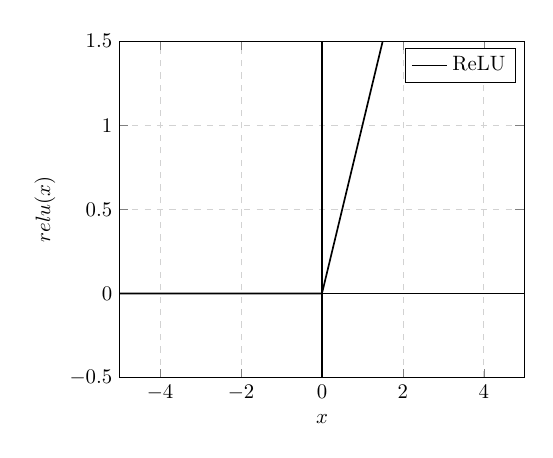
\begin{tikzpicture}[scale=0.75]
		\begin{axis}[
			xlabel=$x$, ylabel=$relu(x)$,
			xmin=-5, xmax=5,
			ymin=-0.5, ymax=1.5,
			grid=major, grid style={dashed, gray!35},
		]
		\addplot[black, samples=500,  thick] {x * (x > 0)};
		
		% This plots a horizontal line from xmin to xmax
		\draw[semithick] (axis cs:\pgfkeysvalueof{/pgfplots/xmin}, 0) -- (axis cs:\pgfkeysvalueof{/pgfplots/xmax}, 0);
		
		% This plots a vertical line from ymin to ymax
		\draw[semithick] (axis cs:0, \pgfkeysvalueof{/pgfplots/ymin}) -- (axis cs:0, \pgfkeysvalueof{/pgfplots/ymax});
		
		\addlegendentry{ReLU}
		\end{axis}
		\end{tikzpicture}
		
		\caption{Rectifier Linear Unit activation function - ReLU.}
		\label{fig:relu}
	\end{figure}